%-------------------------------------------------------------------------------
%	NAME:	report.tex
%	AUTHOR: Connor Beardsmore - 15504319
%	LAST MOD:	01/05/17
%	PURPOSE:	FCC Assignment Report
%	REQUIRES:	NONE
%-------------------------------------------------------------------------------

\documentclass[]{article}
\usepackage[ margin=3cm ]{geometry}
\usepackage{graphicx}
\usepackage{fancyhdr}
\usepackage{float}
\usepackage{hyperref}
\usepackage{transparent}
\usepackage{multicol}
\usepackage{amsmath}
\usepackage[final]{pdfpages}
\usepackage{listings}
\usepackage{color}
\usepackage{algorithmicx}
\usepackage{algpseudocode}
\usepackage{amssymb}
\usepackage[style=chicago-authordate,backend=biber]{biblatex}

\pagestyle{fancy}
\fancyhf{}
\lhead{Connor Beardsmore - 15504319}
\rhead{FCC200}
\lfoot{May 2017}
\rfoot{\thepage}

\pagenumbering{arabic}
\graphicspath{{./images/}}

\addbibresource{bib/references.bib}
\nocite{*}

%-------------------------------------------------------------------------------
% CODE HIGHLIGHTING FOR LISTINGS
\definecolor{codegreen}{rgb}{0,0.6,0}
\definecolor{codegray}{rgb}{0.5,0.5,0.5}
\definecolor{codepurple}{rgb}{0.58,0,0.82}
\definecolor{backcolour}{rgb}{0.99,0.99,0.99}

\lstdefinestyle{mystyle}{
	backgroundcolor=\color{backcolour},   
	commentstyle=\color{codegreen},
	keywordstyle=\color{magenta},
	numberstyle=\tiny\color{codegray},
	stringstyle=\color{codepurple},
	basicstyle=\footnotesize,
	breakatwhitespace=false,         
	breaklines=true,                 
	captionpos=b,                    
	keepspaces=true,                 
	numbers=left,                    
	numbersep=5pt,                  
	showspaces=false,                
	showstringspaces=false,
	showtabs=false,                  
	tabsize=2
}

\lstset{style=mystyle}


%-------------------------------------------------------------------------------
\begin{document}
%-------------------------------------------------------------------------------
% TITLE PAGE

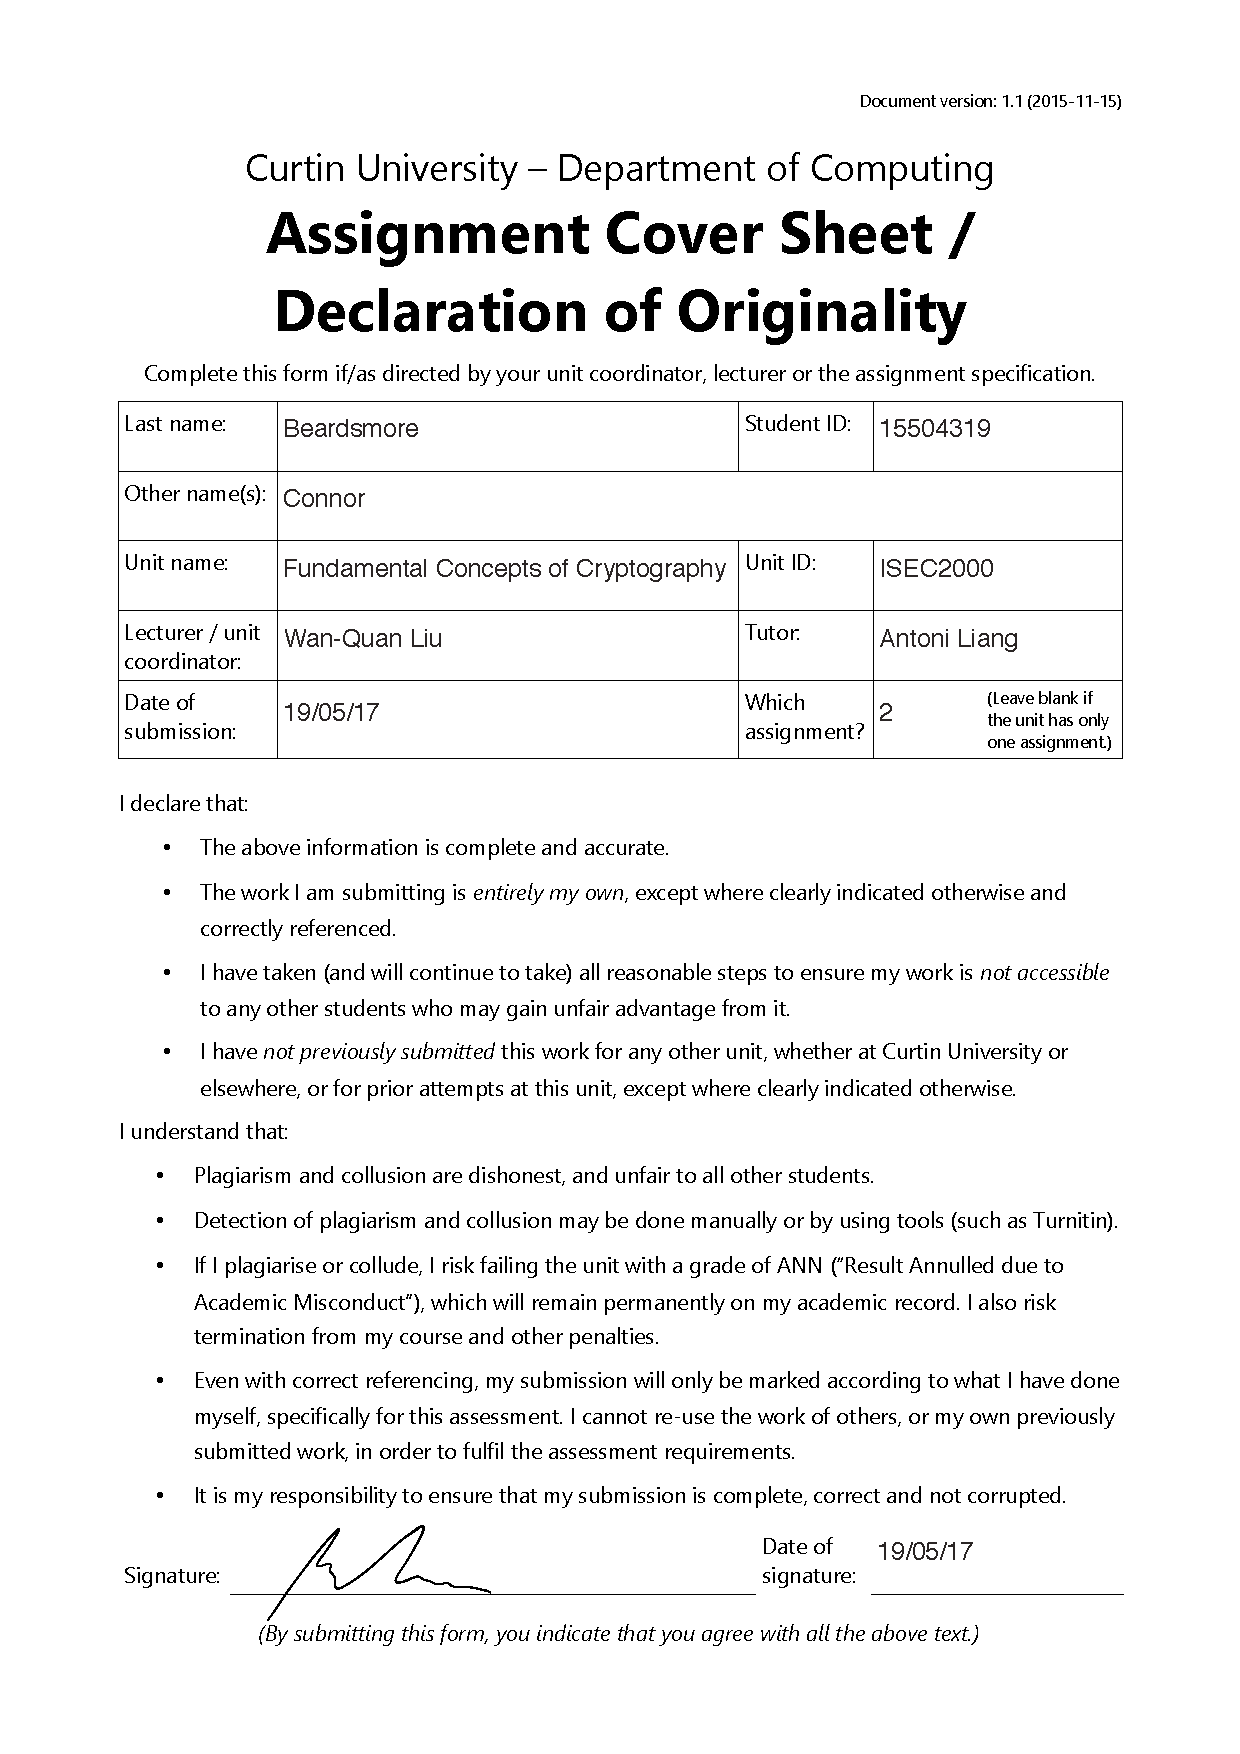
\includepdf[]{./images/cover_page.pdf}

\begin{titlepage}
	\begin{center}
		\vspace*{1cm}
		\LARGE\textbf{FCC200 Report}
		\break
		RSA Cryptosystem Implementation
		\vspace{1cm}
		\break
		\Large\textbf{Connor Beardsmore - 15504319} 
		\vspace{15cm}

		\normalsize
		Curtin University \\
		Science and Engineering \\
		Perth, Australia \\
	    May 2017
	    
	\end{center}
\end{titlepage}

%-------------------------------------------------------------------------------
% BINARY MODULAR EXPONENTIATION
\vspace*{-0.8cm}
\begin{center}
	\section*{Binary Modular Exponentiation}
\end{center}

\lstinputlisting[language=java,linerange={} ]{../../RSA/RSA.java}{}

use the code to print out the value given.

\pagebreak

%-------------------------------------------------------------------------------
% RSA IMPLEMENTATION
\vspace*{-0.8cm}
\begin{center}
	\section*{RSA Implementation}
\end{center}

\subsection*{Original Test File}

\begin{figure}[H]
	
\includegraphics[height=\textheight/6,width=\textwidth]{rsa_plain1.png}
	
\includegraphics[height=\textheight/6,width=\textwidth]{rsa_plain2.png}	
	\caption{RSA Plaintext}
	\centering
\end{figure}

\subsection*{Encrypted Test File}

\begin{figure}[H]
	
\includegraphics[width=\textwidth]{rsa_cipher1.png}
	
\includegraphics[width=\textwidth]{rsa_cipher2.png}	
	\caption{RSA Ciphertext}
	\centering
\end{figure}

\subsection*{Recovered Test File}

\begin{figure}[H]
	
\includegraphics[height=\textheight/6,width=\textwidth]{rsa_plain1.png}
	
\includegraphics[height=\textheight/6,width=\textwidth]{rsa_plain2.png}	
	\caption{RSA Recovered Plaintext}
	\centering
\end{figure}

\pagebreak

%-------------------------------------------------------------------------------
% ADDITIONAL QUESTIONS

\vspace*{-0.8cm}
\begin{center}
	\section*{Additional Questions}
\end{center}

\subsection*{Signature Forgery}

lalasdlasksjdksjs

\subsection*{Birthday Attack}

lalasdlasksjdksjs

\pagebreak

%-------------------------------------------------------------------------------
% RSA CODE

\vspace*{-0.8cm}
\begin{center}
	\section*{RSA Source Code}
\end{center}

\subsection*{RSA.java}
\lstinputlisting[language=java,linerange={} ]{../../RSA/RSA.java}\pagebreak{}

%-------------------------------------------------------------------------------   
% REFERENCES

\break
\setlength\bibitemsep{4\itemsep}
\printbibliography[title={References}]

%-------------------------------------------------------------------------------
\end{document}   
%-------------------------------------------------------------------------------: